\documentclass[11pt, a4paper,titlepage]{article}
\usepackage[a4paper,top=1.5cm,bottom=1.5cm,left=2cm,right=2cm]{geometry}
%% Declaro simbolo
\usepackage[T1]{fontenc}
\newcommand{\rmfont}[1]{{\fontfamily{ptm}\selectfont%
#1}}
\newcommand{\rmfontbf}[1]{{\fontfamily{ptm}\selectfont%
\textbf{#1}}}
\newcommand{\rmfontsc}[1]{{\fontfamily{ptm}\selectfont%
\textsc{#1}}}

%%----------------------------------------------------

	\usepackage[spanish]{babel}
	\selectlanguage{spanish}
   
	\usepackage[utf8]{inputenc} % Aca va el setup para el codigo.
    \usepackage{graphicx}
    \usepackage{upquote}% esto tampoco creo
    \usepackage{amsmath,array,siunitx}
    \newcommand{\vvert}[1]{\left\Vert #1\right\Vert}
    \usepackage{listings}
	\usepackage{mdframed}
	\usepackage{xcolor} 
    \usepackage[utopia]{mathdesign}
    \newcommand{\Matlab}{\rmfont{\sc Matlab}}
    \newcommand{\Adina}{{\sc ADINA}}
    \newcommand{\refp}[1]{(\ref{#1})}
    \newcommand{\unspace}{\!\!\!\!\!\!\!\!\!\!\!\!\!\!\!\!\!\!\!\!}
    \newcommand{\ms}{\ \ \ } %Matrix Spacing
    \newcommand{\di}{\textrm{d}}
    \newcommand{\jac}{\rmfontbf{J}}
    \newcommand{\Djac}{|\;\jac\;|}
    \newcommand{\dNi}{\di N_i}
    \newcommand{\sigmab}{\boldsymbol{\sigma}}
    \newcommand{\varepsilonb}{\boldsymbol{\varepsilon}}
    \newcommand{\Phib}{\boldsymbol{\Phi}}
    \newcommand{\Omegab}{\boldsymbol{\Omega}}
    \newcommand{\COmega}{\boldsymbol{\{ } \Omega \boldsymbol{\} }}
    \newcommand{\CPhi}{\boldsymbol{\{ } \Phi \boldsymbol{\} }}
    \newcommand{\Mme}[1]{\boldsymbol{[}\mathbf{#1} \boldsymbol{]}}
    \newcommand{\Mmes}[1]{\boldsymbol{[}\boldsymbol{ \mathrm{#1} }\boldsymbol{]}}
    \newcommand{\Rme}[1]{\boldsymbol{\lfloor}\mathbf{#1} \boldsymbol{\rfloor}}
    \newcommand{\Cme}[1]{\boldsymbol{\{ }\mathbf{#1} \boldsymbol{\}} }
    \newcommand{\Cmen}[1]{\boldsymbol{\{ }#1 \boldsymbol{\}} }
    \newcommand{\CT}{\Cme{T}}
    \newcommand{\CD}{\Cme{D}}
    \newcommand{\kuD}{\Cmen{k_1^{\dot{D}}}}
    \newcommand{\kdD}{\Cmen{k_2^{\dot{D}}}}
    \newcommand{\ktD}{\Cmen{k_3^{\dot{D}}}}
    \newcommand{\kcD}{\Cmen{k_4^{\dot{D}}}}
    \newcommand{\kuV}{\Cmen{k_1^{\dot{V}}}}
    \newcommand{\kdV}{\Cmen{k_2^{\dot{V}}}}
    \newcommand{\ktV}{\Cmen{k_3^{\dot{V}}}}
    \newcommand{\kcV}{\Cmen{k_4^{\dot{V}}}}
    \newcommand{\MB}{\Mme{B}}
    \newcommand{\MN}{\Mme{N}}
    \newcommand{\ME}{\Mme{E}}
    \newcommand{\MK}{\Mme{K}}
    \newcommand{\MC}{\Mme{C}}
    \newcommand{\Mk}{\Mme{k}}
    \newcommand{\MA}{\Mme{A}}
    \newcommand{\radial}{r}
    \newcommand{\eff}{f}
    \newcommand{\modal}{{_{\Phib}}}
    \newcommand{\dampfact}{\varsigma}
    \newcommand{\spartial}[2]{\ensuremath{\frac{\partial #1}{\partial #2}}}
    
\newmdtheoremenv[% ACA PODES MODIFICAR LAS PROPIEDADES DEL CODIGO {code}
font=\fontsize{12pt}{16pt},
linecolor=black,
leftmargin=-.9cm,%
rightmargin=-.9cm,
backgroundcolor=gray!5,%
innertopmargin=8pt,%
ntheorem]{code}{Codigo}[section]
%-----------------------------------------------------------
% Code

%\newcommand{\feaPP}{codep1.tex}
%\newcommand{\feaSP}{codep2.tex}
%\newcommand{\feaTP}{codep3.tex}
%\newcommand{\annexFile}{annex.tex}
%\newcommand{\feaQP}{codep4.tex}

%No code

\newcommand{\feaPP}{null.tex}
\newcommand{\feaSP}{null.tex}
\newcommand{\feaTP}{null.tex}
\newcommand{\feaQP}{null.tex}
\newcommand{\annexFile}{null.tex}

\begin{document}  %Aqui empieza el documento
\begin{titlepage} %Esta es la caratula
\centering
{\scshape\Huge Elementos Finitos Cheatsheet \par}
\vspace{1cm}

\vspace{2cm}
{\scshape\Large\textbf{Autores} \par}
\medskip %medskip,smallskip,vspace son todos comandos para dejar espacio en blanco entre cosas
 \textsc{55423}

\end{titlepage} %Termina la caratula


\input{\feaPP}
\section{Introduccion al Metodo de los Elementos Finitos}
El análisis o método de elementos finitos (FEA por \textit{finite element analysis}) es usado para obtener una solución numérica de un problema de campo (electrostático, térmico, tensiones). Matemáticamente estos problemas están definidos como ecuaciones diferenciales o como un integral. Ambas expresiones pueden formularse con elementos finitos.

Las ventajas de FEA son

\begin{itemize}
	\item Es aplicable a cualquier problema de campo
	\item No hay restricciones geométricas
	\item No hay restricciones al tipo de cargas o condiciones de borde que se pueden aplicar
	\item Se puede formular para materiales que no son isotrópicos e incluso el tipo de material puede cambiar dentro de un elemento
	\item Se pueden combinar distintos tipos de elementos en un modelos, por ejemplo, unir barras con vigas o incluso con elementos 3D.
	\item La aproximación se puede mejorar fácilmente refinando la malla donde hay gradientes de tensión altos
\end{itemize}

\subsection{Proceso de resolucion}
El primer paso es identificar y \textbf{clasificar} el problema.
\begin{itemize}
	\item Cuales son los fenómenos físicos involucrados?
	\item Depende del tiempo? (estático o dinámico)
	\item Hace falta una resolución iterativa? (no linealidad: radiación, plasticidad)
	\item Que resultados se buscan del análisis
\end{itemize} 

Luego se comienza el \textbf{modelado} del problema.
\begin{itemize}
	\item Se excluyen los detalles superfluos, dejando los esencial para describir el problema con un margen de error adecuado sin complicar las cosas innecesariamente 
	\item Un \textit{modelo geométrico} se convierte en un \textit{modelo matemático} cuando se describe su comportamiento mediante ecuaciones diferenciales y condiciones de borde.\footnote{Un modelo de FEA no es la realidad, es una \textit{simulación}. Difícilmente se obtengan resultados buenos cuando se aplique FEA a un modelo matemático que no refleja la realidad de forma apropiada.}
\end{itemize}
Un modelo matemático es una idealización donde se simplifican la geometría, propiedades del material, cargas y/o condiciones de borde en base del entendimiento del analista acerca lo que tiene (o no) importancia al momento de obtener los resultados requeridos.


Finalmente llega el momento de la \textbf{discretización}. Un modelo matemático se discretiza dividiéndolo en una malla de elementos finitos. De esta forma, un campo continuo es representado como una función partida la cual es definida por una cantidad finita de variables nodales e interpolación dentro de cada elemento.

\subsection{Tipos de error}
Al momento de discretizar se introduce error conocido como \textbf{error de discretización}. Eso sucede porque se aproxima un campo \textit{suave} con una función partida. Aumentar el numero de elementos puede disminuir este error pero nunca eliminarlo.

Aún reduciendo el error de discretización se tendría \textbf{error numérico} porque toda computadora usa números de finita precisión para efectuar aritmética. Este error suele ser mínimo cuando se discretiza de forma adecuada y no se tiene una situación física propensa al \textit{mal condicionamiento}.

Cabe destacar que se introdujo error antes de hacer una sola cuenta! El \textbf{error de modelado} se introduce por necesidad de simplificar el problema. Las cargas puntuales, los soportes fijos y los materiales perfectamente homogéneos no existen en la realidad!


\section{Elementos 1D}


\subsection{Viga 3D de Timoshenko}
\begin{figure}[htb!]
	\centering
	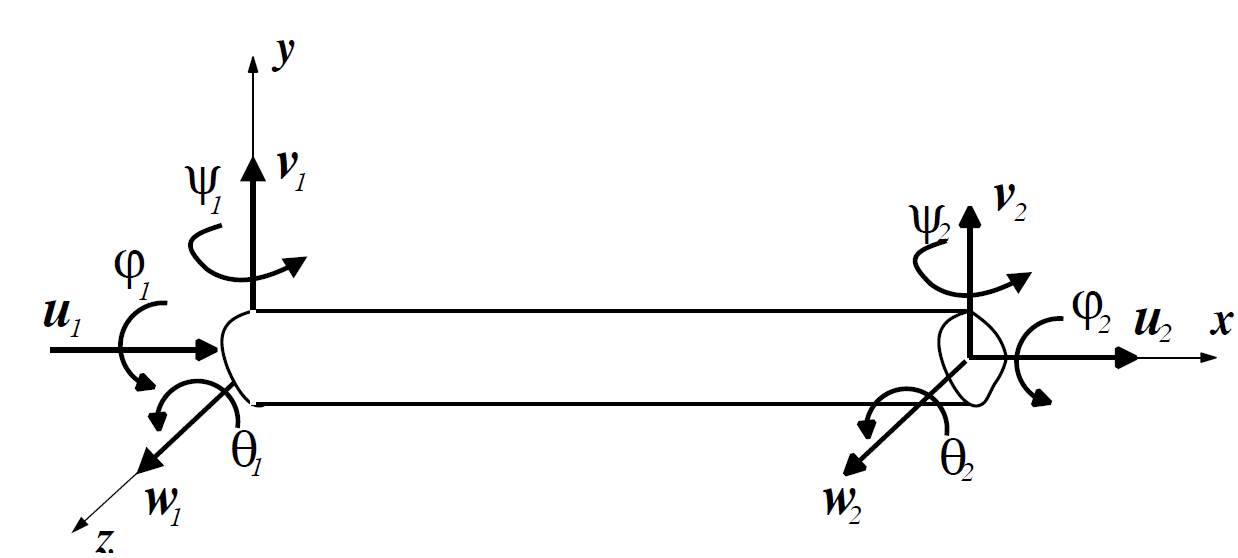
\includegraphics[width=0.6\textwidth]{fig/3dbeam.PNG}
	\caption{Grados de libertad, o \textit{dof}, de una viga 3-D.}
\end{figure}
La viga de Timoshenko 3D tiene las siguientes funciones de forma
\[
\begin{cases}
N_{1}=1-\xi \\
N_2 = \xi \\
H_{v_{1}}=\beta_{y}\left(2 \xi^{3}-3 \xi^{2}+\alpha_{y} \xi+1-\alpha_{y}\right)\\
H_{v_{2}}=\beta_{y}\left(-2 \xi^{3}+3 \xi^{2}-\alpha_{y} \xi\right) \\
H_{w_{1}}=\beta_{z}\left(2 \xi^{3}-3 \xi^{2}+\alpha_{z} \xi+1-\alpha_{z}\right) \\
H_{w_{2}}=\beta_{z}\left(-2 \xi^{3}+3 \xi^{2}-\alpha_{z} \xi\right)\\
H_{\theta_{1}}=L \beta_{y}\left[\xi^{3}+\left(\frac{1}{2} \alpha_{y}-2\right) \xi^{2}+\left(1-\frac{1}{2} \alpha_{y}\right) \xi\right] \\
H_{\theta_{2}}=L \beta_{y}\left[\xi^{3}-\left(1+\frac{1}{2} \alpha_{y}\right) \xi^{2}+\left(\frac{1}{2} \alpha_{y}\right) \xi\right] \\
H_{\psi_{1}}=L \beta_{z}\left[\xi^{3}+\left(\frac{1}{2} \alpha_{z}-2\right) \xi^{2}+\left(1-\frac{1}{2} \alpha_{z}\right) \xi\right] \\
H_{\psi_{2}}=L \beta_{z}\left[\xi^{3}-\left(1+\frac{1}{2} \alpha_{z}\right) \xi^{2}+\left(\frac{1}{2} \alpha_{z}\right) \xi\right] \\
G_{v_{1}}=\frac{6 \beta_{y}}{L}\left(\xi^{2}-\xi\right) \\
G_{v_{2}}=\frac{6 \beta_{y}}{L}\left(-\xi^{2}+\xi\right) \\
G_{w_{1}}=\frac{6 \beta_{z}}{L}\left(\xi^{2}-\xi\right) \\
G_{w_{2}}=\frac{6 \beta_{z}}{L}\left(-\xi^{2}+\xi\right) \\
G_{\theta_{1}}=\beta_{y}\left[3 \xi^{2}+\left(\alpha_{y}-4\right) \xi+1-\alpha_{y}\right] \\
G_{\theta_{2}}=\beta_{y}\left[3 \xi^{2}-\left(\alpha_{y}+2\right) \xi\right] \\
G_{\psi_{1}}=\beta_{z}\left[3 \xi^{2}+\left(\alpha_{z}-4\right) \xi+1-\alpha_{z}\right] \\
G_{\psi_{2}}=\beta_{z}\left[3 \xi^{2}-\left(\alpha_{z}+2\right) \xi\right]
\end{cases}
\]
donde $x$ es la coordenada local sobre la viga:
\[
\xi=\frac{x}{L}, \quad \alpha_{y}=\frac{12 E I_{y}}{k G A L^{2}}, \quad \beta_{y}=\frac{1}{1-\alpha_{y}}, \quad \alpha_{z}=\frac{12 E I_{z}}{k G A L^{2}},\quad  \beta_{z}=\frac{1}{1-\alpha_{z}}
\]
donde $k$ me parece que es la \textit{constante torsional}\footnote{La constante torsional $J_T$ es igual a $I_p$ para secciones de viga circulares. Para perfiles abiertos de paredes delgadas, como por ejemplo un perfil doble T o un perfil `C', $J_T$ es mucho mas chico que $I_p$.} de la viga pero no estoy seguro($J_T$, no es igual al momento de inercia polar: $I_p$).

Estas funciones de forma interpolan los desplazamientos sobre la viga:

\[
\begin{cases}
u=N_{1} u_{1}+N_{2} u_{2} \\
v=H_{v_{1}} v_{1}+H_{\theta_{1}} \theta_{1}+H_{v_{2}} v_{2}+H_{\theta_{2}} \theta_{2} \\
w=H_{w_{1}} w_{1}+H_{\psi_{1}} \psi_{1}+H_{w_{2}} w_{2}+H_{\psi_{2}} \psi_{2} \\
\varphi=N_{1} \varphi_{1}+N_{2} \varphi_{2} \\
\theta=G_{v_{1}} v_{1}+G_{\theta_{1}} \theta_{1}+G_{v_{2}} v_{2}+G_{\theta_{2}} \theta_{2} \\
\psi=G_{w_{1}} w_{1}+G_{\psi_{1}} \psi_{1}+G_{w_{2}} w_{2}+G_{\psi_{2}} \psi_{2}
\end{cases}
\]

para luego calcular los esfuerzos usando las mismas formulas vistas en estatica y resistencia de materiales.
\begin{align*}
M_{z}&=E I_{z} \frac{\di^{2} v}{\di x^{2}}, \qquad V_{y}=\frac{\di M_{z}}{\di x}=E I_{z} \frac{\di^{3} v}{\di x^{3}}, \qquad N_x=A E \frac{u_{2}-u_{1}}{L} \\
\qquad T&=G J_T \frac{\varphi_{2}-\varphi_{1}}{L}, \qquad M_{y}=E I_{y} \frac{\di^{2} w}{\di x^{2}}, \qquad V_{z}=E I_{y} \frac{\di^{3} w}{\di x^{3}}
\end{align*}
donde $J_T$ es la constante torsional de la viga y $A$ es la sección.

La matriz de rigidez se puede obtener
\[ \Mk_{\mathrm{1D}} = \left[\begin{array}{cccccccccccc} X & 0 & 0 & 0 & 0 & 0 & -X & 0 & 0 & 0 & 0 & 0\\ 0 & Y_{1} & 0 & 0 & 0 & Y_{2} & 0 & -Y_{1} & 0 & 0 & 0 & Y_{2}\\ 0 & 0 & Z_{1} & 0 & -Z_{2} & 0 & 0 & 0 & -Z_{1} & 0 & -Z_{2} & 0\\ 0 & 0 & 0 & S & 0 & 0 & 0 & 0 & 0 & -S & 0 & 0\\ 0 & 0 & -Z_{2} & 0 & Z_{3} & 0 & 0 & 0 & Z_{2} & 0 & Z_{4} & 0\\ 0 & Y_{2} & 0 & 0 & 0 & Y_{3} & 0 & -Y_{2} & 0 & 0 & 0 & Y_{4}\\ -X & 0 & 0 & 0 & 0 & 0 & X & 0 & 0 & 0 & 0 & 0\\ 0 & -Y_{1} & 0 & 0 & 0 & -Y_{2} & 0 & Y_{1} & 0 & 0 & 0 & -Y_{2}\\ 0 & 0 & -Z_{1} & 0 & Z_{2} & 0 & 0 & 0 & Z_{1} & 0 & Z_{2} & 0\\ 0 & 0 & 0 & -S & 0 & 0 & 0 & 0 & 0 & S & 0 & 0\\ 0 & 0 & -Z_{2} & 0 & Z_{4} & 0 & 0 & 0 & Z_{2} & 0 & Z_{3} & 0\\ 0 & Y_{2} & 0 & 0 & 0 & Y_{4} & 0 & -Y_{2} & 0 & 0 & 0 & Y_{3} \end{array}\right]\begin{array}{c}
u_1\\
v_1 \\
w_1 \\
\varphi_1 \\
\theta_1 \\
\psi_1 \\
u_2\\
v_2 \\
w_2 \\
\varphi_2 \\
\theta_2 \\
\psi_2 
\end{array} \]
donde 
\begin{align*}
X&=\frac{AE}{L}, \qquad Y_4 = \frac{2EI_z}{L}, \qquad Y_3 = 2Y_4, \qquad Y_2 = \frac{3Y_4}{L} ,\qquad Y_1 = \frac{2Y_2}{L} \\
Z_4 &= \frac{2EI_y}{L}, \qquad Z_3=2Z_4, \qquad Z_2 = \frac{2Z_4}{L}, \qquad Z_1 = \frac{2Z_2}{L}, \qquad S = \frac{G J_T}{L}
\end{align*}



\section{Parcial 2}
Protip: Necesitas saber que fuerza se tiene que hacer para que se mantenga en posición una arista o punto dado cargas térmicas/fuerza? Apoyalo (fix) y mira las reacciones con la carga termica/fuerza.
\subsection{Expresiones útiles}

\begin{align}
    \sigma_{v}&=\sqrt{\sigma_{x}^2+\sigma_{y}^2+\sigma_{z}^2 - \sigma_x \sigma_y-\sigma_x\sigma_z -\sigma_y \sigma_z +3(\sigma_{xy}^2+\sigma_{xz}^2 +\sigma_{yz}^2)} \\
    \sigma_{v}&=\sqrt{\tfrac{1}{2}\left[  (\sigma_{11}-\sigma_{22})^2+(\sigma_{11}-\sigma_{33})^2+(\sigma_{22}-\sigma_{33})^2\right] +3(\sigma_{12}^2+\sigma_{13}^2 +\sigma_{23}^2)}
\end{align}

\begin{equation}
    \lambda = \frac{E \nu}{(1+\nu)(1-2\nu)} \qquad\quad \mu=G=\frac{E}{2(1+\nu)}
\end{equation}

\begin{equation}
\begin{bmatrix}
    \sigma_{xx} \\
    \sigma_{yy} \\
    \sigma_{xy}
\end{bmatrix}
={\frac{E}{1-\nu^2}} 
\begin{bmatrix}
    1 & \nu & 0 \\
    \nu & 1 &0 \\
    0 & 0 & \frac{1-\nu}{2}
\end{bmatrix}
\cdot
\begin{bmatrix}
    \varepsilon_{xx} \\
    \varepsilon_{yy} \\
    2\varepsilon_{xy}
\end{bmatrix}
\end{equation}

\begin{equation}
\begin{bmatrix}
    \sigma_{11} \\
    \sigma_{22} \\
    \sigma_{12}
\end{bmatrix}
={\frac{E}{(1+\nu)(1-2\nu)}} 
\begin{bmatrix}
    1-\nu & \nu &0 \\
    \nu &1-\nu& 0 \\
    0 & 0 & \frac{1-2\nu}{2}
\end{bmatrix}
\cdot
\begin{bmatrix}
    \varepsilon_{11} \\
    \varepsilon_{22} \\
    2\varepsilon_{12}
\end{bmatrix}
\end{equation}

\begin{equation}
    \sigma_{n}=\frac{\sigma_{xx}+\sigma_{yy}}{2}+\left(\frac{\sigma_{xx}-\sigma_{yy}}{2}\right)\cos 2\theta +\tau_{xy}\sin 2\theta 
\end{equation}

\begin{equation}
    \tau_{n}=-\left(\frac{\sigma_{xx}-\sigma_{yy}}{2}\right)\sin 2\theta +\tau_{xy}\cos 2\theta 
\end{equation}

\begin{equation}
    I=\int^1_{-1} \phi(\xi) \di \xi \approx \phi(\xi_1) W_1+\phi(\xi_2) W_2 \ldots \phi(\xi_n) W_n
\end{equation}
\begin{equation}
    I=\int^1_{-1} \int^1_{-1}\phi(\xi,\eta) \di \xi \di \eta\approx \sum_i \sum_j W_i W_j\phi(\xi,\eta) 
\end{equation}



\begin{tabular}{>{$n=$}l<{ \vspace{10pt}}*{13}{c}}
0 &&&&&&&1&&&&&&\\
1 &&&&&&$x$&&$y$&&&&&\\
2 &&&&&$x^2$&&$xy$&&$y^2$&&&&\\
3 &&&&$x^3$&&$x^2y$&&$xy^2$&&$y^3$&&&\\
4 &&&$x^4$&&$x^3y$&&$x^2y^2$&&$xy^3$&&$y^4$&&\\
5 &&$x^5$&&$x^4y$&&$x^3y^2$&&$x^2y^3$&&$xy^4$&&$y^5$&\\
6 &$x^6$&&$x^5y$&&$x^4y^2$&&$x^3y^3$&&$x^2y^4$&&$xy^5$&&$y^6$
\end{tabular}

\begin{figure}
    \centering
    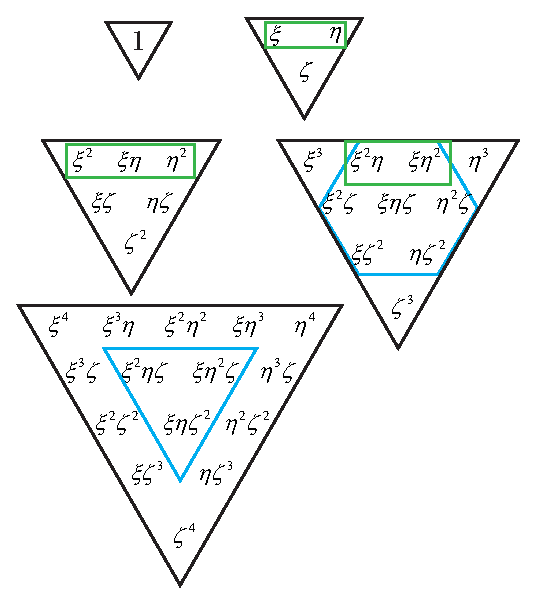
\includegraphics[width=0.5\textwidth]{fig/pascalsTetra.eps}
    \caption{El tetrahedro de Pascal. Los términos de los elementos \textit{serendipidad} están encuadrados.}
    \label{fig:PascalsTetrahedron}
\end{figure}

\subsection{Como obtener cualquier función de forma}
Se define cuantos nodos se va tener por elemento y se los ubica en el espacio $(\xi,\eta)$ que por simplicidad se trataran como $(x,y)$. Con el triangulo de Pascal para polinomios se elige el grado del polinomio y los términos. Luego se resuelve el sistema de ecuaciones $\MN\cdot X= A$ donde $\MN=[N_1\ms N_2 \ms \ldots\ms N_n]$ y $X=[1\ms x\ms y \ms\ldots\ms x^{k-1}y^{k} \ms x^{k}y^{k}]^T$, o algo por el estilo. Se tienen que elegir los grados mas convenientes teniendo en cuenta la simetría y el número de nodos, este ultimo te limita el número de términos posibles por la naturaleza de la interpolación. La matriz $A$ tendrá en su \textbf{espacio fila} el mismo polinomio evaluado en la posición del nodo correspondiente a esa fila.

\[
A=
\begin{bmatrix}
    1 & x_1 & y_1 & \dots  & x_{1}^{k-1}y_1^{k} & x_{1}^{k}y_1^{k} \\
    1 & x_2 & y_2 & \dots  & x_{2}^{k-1}y_2^{k} & x_{2}^{k}y_2^{k} \\
    \vdots & \vdots & \vdots & \ddots & \vdots& \vdots \\
    1 & x_n & y_n & \dots  & x_{n}^{k-1}y_n^{k} & x_{n}^{k}y_n^{k}
\end{bmatrix}
\]
Luego, las funciones de forma $\MN$ se pueden obtener así: $\MN=X^{-1} A$

\subsection{Elementos isoparamétricos}
\begin{itemize}
    \item Un elemento que no esta distorsionado (sigue siendo rectangular) tiene $J$ constante
    \item Cuidado con modo espurio. Ver tabla 6.8-1 pg. 226 el tema de full/reduced integration.
    \item Todo sobre como cargar tu elemento isoparam. en pg. 228
    \item 
\end{itemize}

\begin{figure}[htb!]
    \centering
    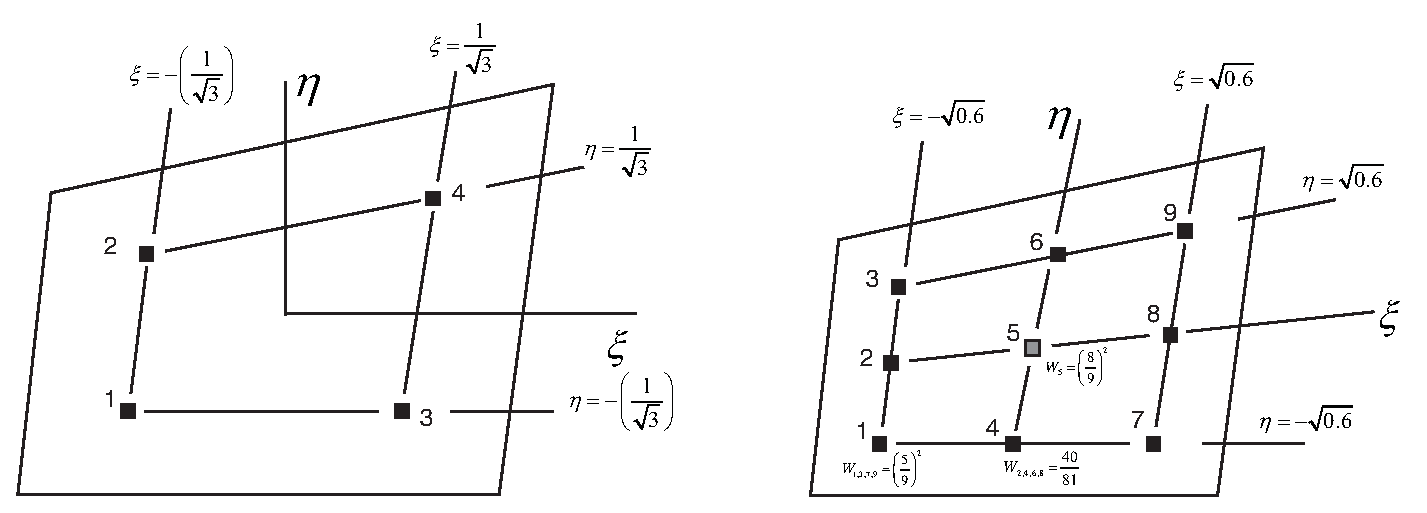
\includegraphics[width=12cm]{fig/gauss_n3.eps}
    \caption{Puntos gauss para ordenes $n=2$ y $n=3$. El peso para $n=2$ es igual en todos los puntos $W_i=1$}
    \label{fig:gauss_n3}
\end{figure}
\subsection{Ejemplo elemento exótico}
\subsubsection*{Matriz de Rigidez}
Imaginemos un elementos Q5 cuadrado de $2\times2$ con espesor $t$  (igual al Q4 con un nodo en su centro). Si fuéramos a obtener las funciones de formas de dicho elemento quedarían iguales para $(x,y)$ y para $(\xi,\eta)$ por las dimensiones usadas. La funcionalidad que uno estaría tentado a seleccionar sería $[1,\ x, \ y,\ x^2, \ y^2 ]$, pero está trae problemas inesperados debido a que tiene varias soluciones en la interpolación. Como nuestra prioridad siempre es mantener la simetría la funcionalidad será $[1,\ x,\ y,\ xy,\ x^2y^2 ]$.  Tomando el orden de la figura \ref{fig:elemq5}.
\[
\MN=\left[\begin{array}{ccccc} \frac{x^2\,y^2}{4}+\frac{x\,y}{4}-\frac{x}{4}-\frac{y}{4}, & \frac{x^2\,y^2}{4}-\frac{x\,y}{4}+\frac{x}{4}-\frac{y}{4}, & \frac{x^2\,y^2}{4}+\frac{x\,y}{4}+\frac{x}{4}+\frac{y}{4}, & \frac{x^2\,y^2}{4}-\frac{x\,y}{4}-\frac{x}{4}+\frac{y}{4}, & 1-x^2\,y^2 \end{array}\right]
\]

Llegado a este punto nos interesa obtener la matriz de rigidez. Si queremos lograr \emph{``full integration"} deberíamos usar Gauss orden $n=3$ según $2n-1\geq O\left(\MB^T \ME \MB \right)$. $\MB$ es el \textit{strain-deformation matrix}. El producto $\MB^T \ME \MB$ da un polinomio de orden 6 ($\MB$ tiene el mismo orden que la derivada de $\MN$). De esta forma nos aseguramos que nuestro resultado va ser exacto para el elemento sin distorsionar.

Para esté ejemplo, no se pide \emph{full integration} entonces no pasa nada si queremos \emph{underintegrate}. Usamos Gauss orden $n=2$. 

\begin{figure}[htb!]
    \centering
    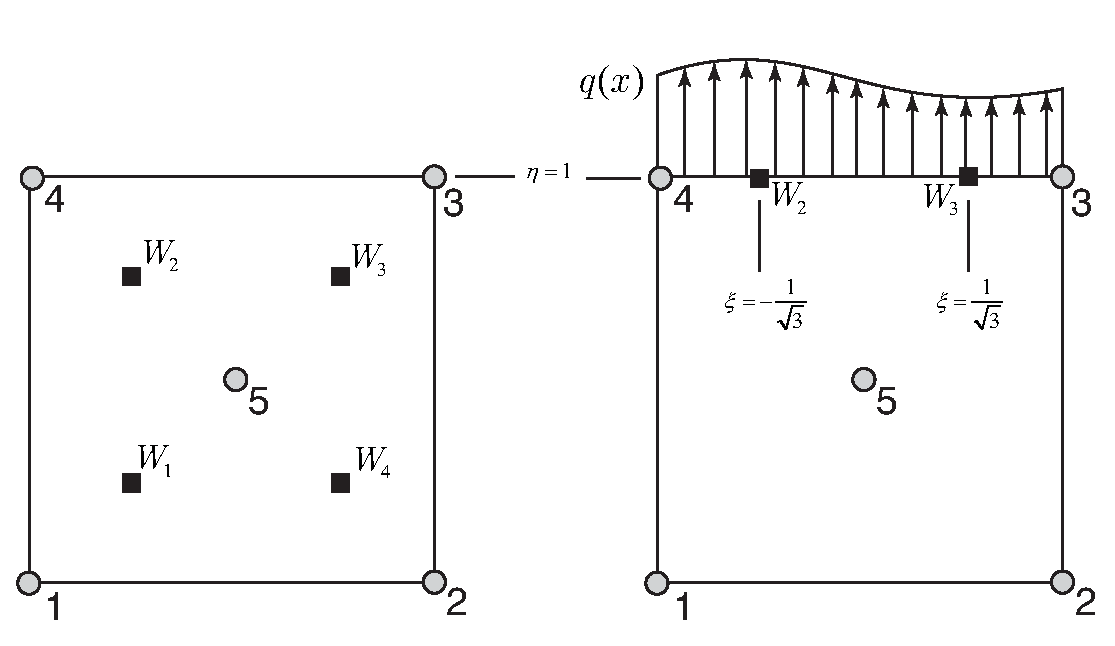
\includegraphics[height=5cm]{fig/exoticElement.eps}
    \caption{Elemento Q5 rectangular.}
    \label{fig:elemq5}
\end{figure}

La rigidez de un elemento está dada por 


\begin{equation} \label{eq:RigidezElemento}
    \Mk=\int \MB^T \ME \MB \di V
\end{equation}
para un elemento plano la ecuación anterior es
\[
\Mk_{\mathrm{2D}}=\iint \MB^T \ME \MB t \di x \di y=\int^1_{-1}\int^1_{-1} \MB^T \ME \MB t \ \Djac \  \di\xi  \di\eta
\]
donde $\MB$ es la matriz deformación-desplazamiento del elemento, $\ME$ es la matriz constitutiva, y $\Djac$ es el determinante de la matriz Jacobiana, el cual se le suele decir simplemente el Jacobiano.

Este ultimo se calcula a partir de la derivada de las funciones de forma $ $

\subsubsection*{Cargas 2-D}
La ecuación que rige como se cargan elementos, siendo $\Cme{r}$ las cargas nodales, $\Cme{F}$ fuerzas volumétricas, $\CPhi$ fuerzas de tracción superficiales, $\Cme{\varepsilonb_0}$ las deformaciones iniciales y $\Cme{\sigmab_0}$ las tensiones iniciales (pg. 228)
\begin{equation} \label{eq:CargasGenerales}
    \Cme{r}=\int \MN^T \Cme{F} \di V +\int \MN^T \CPhi \di S+\int \MB^T \ME \Cme{\varepsilonb_0} \di V- \int \MB \Cme{\sigmab_0} \di V
\end{equation}
\textbf{Carga de linea}. Si el elemento está cargado sobre la linea 4-3 con una distribuida $q(x)$ (en [\si{\newton \per \meter}]) entonces procedemos de la siguiente manera según el segundo término de \refp{eq:CargasGenerales}: 

\begin{align}
    r_{xi}&=\int^1_{-1}N_i (\tau \jac_{11}- \sigma \jac_{12})t\di \xi \\
    r_{yi}&=\int^1_{-1}N_i (\sigma \jac_{11}+\tau \jac_{12})t \di \xi 
\end{align}
    donde $\sigma$ es la solicitación normal a la superficie y $\tau$ es la tangencial. Para la fuerza sobre el nodo 4 se tiene
    
    $$r_{y4}= N_4(\xi_2)t\left[\sigma(\xi_2)\; \jac_{11}+\tau(\xi_2)\; \jac_{12}\right] \cdot W_2 + N_4(\xi_3)t\left[\sigma(\xi_3)\; \jac_{11}+\tau(\xi_3)\; \jac_{12}\right]\cdot W_3 $$

    Si consideramos que solo hay una \emph{carga distribuida de linea} a tracción/compresión como indica la figura \ref{fig:elemq5}, se reduce la ecuación anterior
    
    $$ r_{y4} = N_4(\xi_2)\;\jac_{11}\;q(\xi_2) + N_4(\xi_3)\;\jac_{11}\;q(\xi_3) =N_4\;q \;\jac_{11}\Big|_{\xi_2} + N_4\;q\; \jac_{11}\Big|_{\xi_3} $$
    similarmente $r_{y3} = N_3\;q \;\jac_{11}\big|_{\xi_2} + N_3\;q\; \jac_{11}\big|_{\xi_3} $ donde la matriz Jacobiana también se evalúa para cada punto de Gauss!
    
    \textbf{Carga volumétrica}. 
\subsubsection*{Tensiones}
    \begin{itemize}
        \item Las tensiones en los nodos suele ser de mayor interés que sobre los puntos de gauss (mas comprometidas, permiten estimar error)
    \end{itemize}
    \clearpage
 \input{\feaSP}
\section{Parcial 3}

\subsection{Axisimetría}
Resuelvo problema 3-D en el plano. Los resultados son por cada unidad radian. Como sigo teniendo dos grados de libertad tengo las mismas funciones de forma. Cambia mi operador derivada.
\[
\begin{Bmatrix}
    \sigma_\radial \\
    \sigma_\theta \\
    \sigma_z \\
    \tau_{z\radial}
\end{Bmatrix}
= \frac{(1-\nu)E}{(1+\nu)(1-2\nu)}
\begin{bmatrix}
   1 & \eff & \eff & 0 \\
    & 1 & \eff & 0 \\
    & & 1 & 0 \\
    \textrm{sim.}\unspace& & & g 
\end{bmatrix}
\left(
\begin{Bmatrix}
\varepsilon_\radial \\
\varepsilon_\theta \\
\varepsilon_z \\
\gamma_{\radial z}
\end{Bmatrix}
-
\begin{Bmatrix}
\alpha T\\
\alpha T \\
\alpha T \\
0
\end{Bmatrix}
\right)
\]
donde 
\[
f=\frac{\nu}{1-\nu}\qquad \quad \textrm{y}\quad \qquad g=\frac{1-2\nu}{2(1-\nu)}
\]

Una carga puntual $P$ aplicada sobre un elemento axisimétrico no tiene el mismo significado físico que en elementos plane stress/strain. 
\[
P=2\pi rq
\]
donde $q$ es la carga distribuida en [N/m], $r$ es la distancia al eje de revolución y $2 \pi$ es el resultado de integrar la fuerza distribuida sobre $\theta$. 

\[
\Cme{r_e} = \int\int_{-\pi}^{\pi} \MN^T \begin{Bmatrix}
    \rho r \omega ^2 \\
    0
\end{Bmatrix} r \di \theta \di A
\]

\subsection{Constraints}
Rigid Links


\subsection{Subestructuras}
\[
\begin{bmatrix}
    K_{AA} & K_{AB} \\
    K_{BA} & K_{BB}
\end{bmatrix}
\begin{bmatrix}
    D_A \\
    D_B
\end{bmatrix}
= \begin{bmatrix}
    R_A \\
    R_B
\end{bmatrix}
\]

\[ 
D_B = K_{BB}^{-1} (R_B - K_{BA}D_A)
\]
\[
D_A =K_{AA}^{-1}(R_A-K_{AB}D_B)
\]

\subsection{Pitfalls}
\subsubsection*{\Matlab{}}
\begin{itemize}
    \item Antes de aplicar carga distribuida, verificar la orientación del elemento con sus nodos ($\xi,\eta$)
    \item
\end{itemize}
\subsection{Error}
Tipos de error:
\begin{itemize}
    \item Modelado
    \item Bugs
    \item Error de usuario
    \item Error de discretización
    \item Error de redondeo/truncado
    \item Error de manipulación 
    \item Error numérico (combinación de los dos anteriores)
\end{itemize}

Cálculo Tensiones en puntos superconvergencia (Gauss orden 1 para Q4, y Gauss orden 2 aproxima para Q8).

Extrapolo tensiones superconvergentes a los nodos ($\sigma^*$).

Energía de deformación.

Se suele requerir que $\eta\leq 0,05$
\[
\vvert{U}^2 = \sum^m_{i=1}\int_{v_e} \Cme{\varepsilonb}_i^T \ME \Cme{\varepsilonb}_i \di V
\]
\[
\vvert{e}^2=\sum_{i=1}^m \int_{v_e} \left( \Cme{\varepsilonb^*}_i - \Cme{\varepsilonb}_i\right)^T \ME \left( \Cme{\varepsilonb^*}_i - \Cme{\varepsilonb}_i\right) \di V
\]

\[
\vvert{e}^2=\sum_{i=1}^m \int_{v_e} \left( \Cme{\sigmab^*}_i - \Cme{\sigmab}_i\right)^T \ME ^{-1} \left( \Cme{\sigmab^*}_i - \Cme{\sigmab}_i\right) \di V
\]

\[
\eta = \sqrt{\frac{\vvert{e}^2}{\vvert{e}^2+\vvert{U}^2}}
\]




\input{\feaTP}
\subsubsection*{\Adina}
\begin{figure}[htb!]
    \centering
    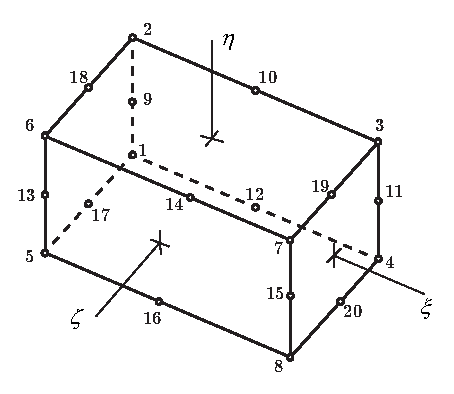
\includegraphics[width=.6\textwidth]{fig/H20numbering.eps}
    \caption{Numeración de nodos H20 en \Adina (Ejes sugeridos)}
    \label{fig:H20numbering}
\end{figure}

\subsection{Formulacion elemento Hexahedro de 8 nodos}
\newcommand{\dof}{\ensuremath{\mathrm{dof}}}
El modelado con elementos isoparametricos hexaedros de 8 nodos es un buen punto de partida para comenzar a manejar los elementos finitos en 3 dimensiones. Un codigo hecho para obtener $\MK$ con elementos H8 se adapta con facilidad para los H20.

Cada nodo tendrá $3$ grados de libertad, dándonos $24$ \dof{} por elemento. El elemento H20 de la figura \ref{fig:H20numbering} esta planteado de tal forma que los primeros nodos del 1 al 8 son los nodos del H8 que se va formular a continuación.

La funcionalidad a usar es la siguiente

\[
X_{\mathrm{H8}} = \left[1, \xi, \eta, \zeta, \xi \eta, \xi \eta, \eta \zeta, \xi \eta \zeta \right]
\]


y la matriz constitutiva para el espacio 3D con 3 \dof{} por nodo se escribe:

\begin{equation}
	\ME =\left[\begin{array}{cccccc} 2\,G+\lambda  & \lambda  & \lambda  & 0 & 0 & 0\\ \lambda  & 2\,G+\lambda  & \lambda  & 0 & 0 & 0\\ \lambda  & \lambda  & 2\,G+\lambda  & 0 & 0 & 0\\ 0 & 0 & 0 & G & 0 & 0\\ 0 & 0 & 0 & 0 & G & 0\\ 0 & 0 & 0 & 0 & 0 & G \end{array}\right] \qquad \ME^{-1}=\frac{1}{E}\left[\begin{array}{cccccc} 1 & -\nu  & -\nu  & 0 & 0 & 0\\ -\nu  & 1 & -\nu  & 0 & 0 & 0\\ -\nu  & -\nu  & 1 & 0 & 0 & 0\\ 0 & 0 & 0 & f & 0 & 0\\ 0 & 0 & 0 & 0 & f & 0\\ 0 & 0 & 0 & 0 & 0 & f \end{array}\right]
\end{equation}
donde $\lambda = \frac{E \nu}{(1+\nu)(1-2\nu)}$ y $G=\frac{E}{2(1+\nu)}$ y $f = 2+2\nu$.

\subsubsection{Formulación elementos}
El jacobiano tiene la forma
\[
\jac=
\left[\begin{array}{lll}\spartial{x}{\xi} & \spartial{y}{\xi}  & \spartial{z}{\xi}  \\ \spartial{x}{\eta}  &\spartial{y}{\eta}  &\spartial{z}{\eta} \\\spartial{x}{\zeta} & \spartial{y}{\zeta} &\spartial{z}{\zeta}\end{array}\right]
\]
pudiendo ser calculado de la siguiente forma

\begin{equation}
	\jac = \begin{bmatrix}
	\frac{\partial}{\partial \xi} \MN \\
	\frac{\partial}{\partial \eta} \MN \\
	\frac{\partial}{\partial \zeta} \MN 
	\end{bmatrix}
	\cdot 
\left[\begin{array}{lll}{x_{1}} & {y_{1}} & {z_{1}} \\ {x_{2}} & {y_{2}} & {z_{2}} \\ {x_{3}} & {y_{3}} & {z_{3}} \\ {x_{4}} & {y_{4}} & {z_{4}} \\ {x_{5}} & {y_{5}} & {z_{5}} \\ {x_{6}} & {y_{6}} & {z_{6}} \\ {x_{7}} & {y_{7}} & {z_{7}} \\ {x_{8}} & {y_{8}} & {z_{8}}\end{array}\right]
\end{equation}
donde la primer matriz termina siendo $3\times8$ para un elemento H8. La segunda matriz son las posiciones \textit{globales} de los nodos del elemento. El jacobiano se puede entonces utilizar para calcular

\begin{equation}
	\Mme{\partial N}=\left[\begin{array}{l} \frac{\partial}{\partial x}\MN  \\ \frac{\partial}{\partial y} \MN  \\ \frac{\partial}{\partial z} \MN  \end{array}\right]=\jac^{-1}\left[\begin{array}{l}\frac{\partial}{\partial \xi} \MN \\
	\frac{\partial}{\partial \eta} \MN \\ 
	\frac{\partial}{\partial \zeta} \MN \end{array}\right]
\end{equation}
con lo obtenido se puede calcular la matriz $\MB$.

La matriz \textit{strain-deformation} queda
\[
\MB = \begin{bmatrix}
B_1 &B_2 &B_3 &B_4 &B_5 &B_6 &B_7 &B_8
\end{bmatrix}
\]
donde
\begin{equation}
B_{i}=\left[\begin{array}{ccc}{\partial N_{i} / \partial x} & {0} & {0} \\ {0} & {\partial N_{i} / \partial y} & {0} \\ {0} & {0} & {\partial N_{i} / \partial z} \\ {0} & {\partial N_{i} / \partial z} & {\partial N_{i} / \partial y} \\ {\partial N_{i} / \partial z} & {0} & {\partial N_{i} / \partial x} \\ {\partial N_{i} / \partial y} & {\partial N_{i} / \partial x} & {0}\end{array}\right]
\end{equation}

Finalmente un calcula la rigidez del elemento usando \eqref{eq:RigidezElemento}.






\section{Finitos II}
\begin{equation} \label{eq:vibraciones}
	\Mme{M}\Cme{\boldsymbol{\ddot{\mathrm{D}}}} + \Mme{C}\Cme{\boldsymbol{\dot{\mathrm{D}}}}+\Mme{K} \Cme{D} =\Cme{R}
\end{equation}
Amortiguamiento $\Mme{C} = \alpha \Mme{M}+\beta \Mme{K}$ cede una matriz no diagonal. Se complica la resolución. Existen dos otros modelos que tratan con una matriz $\Mme{C\modal}$ diagonal donde las ecuaciones se desacoplan.


Amortiguamiento Modal: Se elige un $\dampfact$ para cada modo
\begin{equation}
\Mme{C\modal}=\left[ \begin{array}{ccc}{2 \omega_{n} \dampfact_{n}} & {0} & {0} \\ {0} & {\ddots} & {0} \\ {0} & {0} & {2 \omega_{1} \dampfact_{1}}\end{array}\right]
\end{equation}

Amortiguamiento proporcional. Se basa el análisis 

\begin{equation}
	\Mme{C\modal} = \Mme{\Phib}^T ( \alpha \Mme{M}+\beta \Mme{K})\Mme{\Phib} = \alpha \delta \Mme{I} +\beta \Mme{\Omegab^2}
\end{equation}

Si se quiere estudiar un rango de frecuencias de excitación tal que $\omega_{\mathrm{exc}}\in [\omega_1, \omega_2]$ y eligiendo dos valores de damping para ambas frecuencias $\dampfact_1$ y $\dampfact_2$ se tiene:
\begin{align*}
\alpha &= 2\omega_1 \omega_2 (\dampfact_1 \omega_2 -\dampfact_2 \omega_1)/(\omega_2^2 - \omega_1^2) \\ \beta &= 2(\dampfact_2\omega_2 -\dampfact_1 \omega_1)/(\omega_2^2 - \omega_1^2)
\end{align*}

Una vez obtenida $\Mme{C\modal}$ se pueden obtener los desplazamientos modales $\Cme{Z}$. Tome en cuenta que debido a la diagonalidad de $\Mme{\Omegab^2}$ y $\Cme{R\modal }$ se desacoplan las ecuaciones de \ref{eq:vibraciones} y por ende se pasa a tratar dichas matrices diagonales como vectores columnas. Una vez desacopladas se tiene
 \[\Cme{\boldsymbol{\ddot{\mathrm{Z}}}}+2\COmega \Cme{C\modal} \Cme{\boldsymbol{\dot{\mathrm{Z}}}} + \COmega^2 \Cme{Z} = \Cme{R\modal} \]
\[
\Cme{Z} = \frac{\Cme{R\modal }}{{\COmega}^2 \sqrt{(1-\chi^2)^2 + (2 \Cme{C\modal} \chi)^2}}
\]
donde $\chi = \frac{\omega_{\mathrm{exc}}}{\COmega}$. 



\subsection{Sine Sweep}
A medida que la frecuencia de excitación aumenta la \textit{amplitud del sistema disminuye}\footnote{Excepto en cercanías de una frecuencia natural}. Es interesante pensar que si aumentara no tendría sentido buscar las frecuencias naturales porque estas son caracterizadas por un máximo de amplitud. Las curvas del barrido de frecuencia son decrecientes en lejanía de una frecuencia natural porque para una fuerza cíclica $F(t)=F_0\sin \omega t$ el tiempo que actúa en una dirección es inversamente proporcional a la frecuencia. Por ende la estructura no tiene tiempo para moverse lejos antes de que se invierta la dirección de la fuerza.



\section{Apuntes Segundo Parcial}

Es cuasiestatico cuando la deformacion avanza 

Cargas armonicas: Analizo respuesta de la estructura ante cada modo. 

Aumentar damping disminuye la amplitud del motor, pero a la vez lo que le otorga damping se convierte rigido y toma reacciones.

Para simular transitorio podemos usar la descomposicion modal con metodos numericos usando runge kutta... porque ahora tengo una particular... la funcion 

Ahora pueden variar de cualquier manera:
\[
D=D(x,y,z,t) = N(x,y,z)D(t)
\]

Desarrollamos $D$ en serie Taylor.

$f(x_0+\Delta x)= f(x_0) + f'(x_0) \Delta x +\tfrac{1}{2}...$

Con las ecuaciones de taylor despejadas para $n+1$ y $n-1$ puedo adivinar el futuro con el presente (y pasado).
\[
\{D\}{n+1}=\{D\}{n-1}+2 \Delta t\{\dot{D}\}_{n}
\]

Sin conocer $\dot{D}_{n}$ esta dificil... uso taylor otra vez!

\[
\left[\frac{M}{\Delta t^{2}}+\frac{C}{2 \Delta t}\right]\{D\}{n+1}=\left\{R^{e x t}\right\}{n}-[K]\{D\}{n}+\frac{2}{\Delta t^{2}}[M] \} D{n}-\left[\frac{M}{\Delta t^{2}}-\frac{C}{2 \Delta t}\right]\{D\}_{n-1}
\]

donde $\left\{ R^{e x t}\right\}$ puede ser una función en el tiempo también! Una funcion heaviside excita TODOS los modos.

Optimización: No hay mucho que se pueda hacer. Es super complicated

Se presentan al lector dos formas de resolver la siguiente ecuacion:
\[
\left\{\begin{array}{l}{[M] \dot{V} \}+[C] V \}+[K]\{D\}=\left\{R^{\text {ert}}\right\}} \\ {\{\dot{D}\}=\{V\}}\end{array}\right.
\]
Integración directa
\begin{align*}
	\begin{cases}
	\Cme{V}^{n+1}&=\Cme{V}^n + \frac{\Delta t}{2}  \Mme{M}^{-1}\left(\Cme{R^{\mathrm{ext}}} - \MC \Cme{V} - \MK \Cme{D} \right) \\
	\Cme{D}^{n+1}&=\Cme{D}^n + \frac{\Delta t}{2} \Cme{V}
	\end{cases}
\end{align*}


RUNGE KUTTA

Tengo que resolver las dos ecuaciones simultáneamente
\[
\begin{cases}
	\Cme{V}^{n+1}=\Cme{V}^n + \frac{\Delta t}{6} \left( \kuV + 2\kdV + 2\ktV + \kcV \right) \\
	\Cme{D}^{n+1}=\Cme{D}^n + \frac{\Delta t}{6} \left( \kuD + 2\kdD + 2\ktD + \kcD \right) \\
\end{cases}
\]
donde 
\begin{align*}
	\begin{cases}
	\kuV &= \Mme{M}^{-1} \left( \Cme{R^{\mathrm{ext}}}^n - \MC \Cme{V}^n - \MK \Cme{D}^n  \right) \\
	\kuD &= \Cme{V}^n \\\hline
	\kdV &= \Mme{M}^{-1} \left( \Cme{R^{\mathrm{ext}}}^{n+\frac{1}{2}} - \MC \left(\Cme{V}^n + \frac{\Delta t}{2} \kuV \right) - \MK \left( \Cme{D}^n + \frac{\Delta t}{2} \kuD \right)  \right) \\
	\kdD &= \Cme{V}^n + \frac{\Delta t}{2} \kuV \\	\hline
	\ktV &= \Mme{M}^{-1} \left( \Cme{R^{\mathrm{ext}}}^{n+\frac{1}{2}} - \MC \left(\Cme{V}^n + \frac{\Delta t}{2} \kdV \right) - \MK \left( \Cme{D}^n + \frac{\Delta t}{2} \kdD \right)  \right) \\
	\ktD &= \Cme{V}^n + \frac{\Delta t}{2} \kdV \\	\hline
	\kcV &= \Mme{M}^{-1} \left( \Cme{R^{\mathrm{ext}}}^{n+1} - \MC \left(\Cme{V}^n + \Delta t \ktV \right) - \MK \left( \Cme{D}^n + \Delta t \ktD \right)  \right) \\
	\kcD &= \Cme{V}^n + \Delta t \ktV
	\end{cases}
\end{align*}


Espectro de respuesta


Gráfico $\ddot{u}$--$\omega$ muestra las cargas que podría estar sometido tu sistema.

A frecuencias mas altas la diferencia entre las Z es mayor:

\[
S_{i}=\frac{Z_{i}^{\text { mâx }}}{Z_{i}^{\text { st }}}
\]

Ataco el sistema con un ``Paquete`` de cargas y cada modo responde de su propia forma. Este metodo Sebas le dice Random. Se suele usar para sistemas tipo placas en satelites, donde tenes todas las plaquetas vibrando y no conoces que esta pasando ahi. Para estructuras no tanto porque son más estables y se conoce mejor que puede llegar a ser el modo de vibración porque los modos de vibracion estan bien separados-> cosa que no es verdad en satelites. 

\[
\mathrm{D}(\mathrm{t}){\mathrm{j}}=[\Phi]\{\mathrm{Z}(\mathrm{t})\}=\sum{\mathrm{j}} \Phi_{\mathrm{ji}} Z_{\mathrm{i}}(\mathrm{t})=\sum_{\mathrm{j}} \Delta_{\mathrm{ji}}(\mathrm{t})
\]



Voy a tener un desplazamiento máximo cuando los modos esten todos en su máximo... pero eso sucede cuando están en fase, cosa que nunca sucede porque siempre hay algun desfasaje. Hay criterios para determinar el desplazamiento máximo, una incluye sumando la primer autoforma que es la más grande y luego sumando cuadrados mínimos de las otras. Con esto te cubris de la tensión que podría llegar a ocurrir ().


\section{No linealidad}
Metodo variacional: Lo que buscamos es un estado de energia minima para el sistema, y como para obtener la energia tenemos que integrar se requiere integrar todo el sistema. Buscamos un punto donde el funcional sea estable. Decimos que toda la energia interna es igual al trabajo externo. 

Formula resuelta en Resistencia de materiales
\[
E I \frac{d^{4} v}{d x^{4}}-q=0
\]

Formula resuelta en elementos finitos
\[
\Phi=\int_{0}^{L} \frac{E I}{2}\left(\frac{d^{2} v}{d x^{2}}\right)^{2}-q v d x \rightarrow \delta \Phi=0
\]

Para resolver variacionalmente necesitamos un potencial. Necesitamos saber como se almacena la energia. Con plasticidad pierdo energia, se entrega a la pieza de la forma de deformacion permanente. 

Segun el principio de los trabajos virtuales. Lo que en verdad estamos escribiendo es un equilibrio de fuerzas, porque me estoy preguntando el estado final y si esta en equilibrio haciendo el calculo "si me muevo un cachito cuanto trabajo hago?". Entonces no estoy mirando los procesos disipativos! 

Como hago para los fluidos si quiero aplicar PTV a fluidos? Tenes que plantear el Principio de trabajo virtual, lo mismo pero ahora con el tiempo ahi metido.


Hu-Washizu
\[
\int_{V^{e}}\left[\frac{1}{2} \varepsilon^{T} C \varepsilon-\sigma^{T} \varepsilon+\sigma^{T}(\nabla u)-\overline{p}^{T} u\right] d V-\int_{S_{\sigma}^{e}} \overline{T}^{T} u d S
\]
Separa parte elastica, deformaciones iniciales,  etc. Sebas lo uso para que elementos Q6 pasen el Patch test.

\subsection{Residuos Ponderados}
Y si no tengo la fisica? Balance de una viga de seccion $A$ con carga $q$.
\[
A \frac{\partial \sigma_{x}}{\partial x}+q=0
\]

Pero el ultimo elemento de la viga esta sometido a carga $P$. La condicion de borde natural es:
\[
A E \frac{\partial u}{\partial x}=P
\]
Una condicion de borde comun seria $u=0$ sobre el empotramiento.

Soy vidente y digo que $\widetilde{u}=a_{1} x+a_{2} x^{2}$. el mon~o es por aproximada

Metiendolo en el PDE obtengo ecuaciones y resuelvo por los $a$. Si tenes mucha suerte los Residuos te dan cero tenes mucha suerte y lo que tenes en tus manos es una solucion al sistema. Wl residuo te dice cuanto error estas cometiendo. $R_s=0$ vale cero siempre porque es una condicion que impusimos.


Que hago? Calculo para que en $x=x_0$ el residuo valga cero (Sebas dice en $x=L/3$).  

Hago una grilla de puntos y pido que se cumpla la ecuacion en ellos.

Si planteo que el integral de $R$ valga cero entonces como que coloc un punto en $x=L/2$. Colocacion por puntos, es rapido y medio chotengui, pero anda bien en una malla fina. 

Metodo cuadrado minimos busca reducir el $R$ violentamente. Integro el residuo al cuadrado mas el residuo en la condicion de borde al cuadrado multiplicado por un factor que podes multiplicarlo por grandes numero par a que se cumpla forzadamente. $1/L^2$ te da unidades correctas para dicho factor $\alpha$ 

Galerkin: Las condiciones de borde naturales se llaman asi  porque no las ves, pero estan metidas ahi en la ecuacion. a diferencia de las comunes quelas eligo yo.

Porque co`no meto una funcion a multiplicar el residuo? Porque esta proyectando de tal forma de que valga cero. Si soy inteligente para proectar voy a lograr que las proyecciones sean nulas.

Al vector puedo descomponerlo en dos direcciones. Proyectamos tal que nos de cero en ciertas direcciones. Depende de cuantos coeficientes pusistes, proyectas tantas veces. 

En la filmina 12 Sebas reemplaza $=\int_{V}-\frac{\partial W_{i}}{\partial x} \frac{\partial u}{\partial x} d v$ y reemplaza cada peso correpsondiente.

Galerkin 1D pg 13: Proyecto las funciones de forma del nodo respecto las otras y si misma. vector de cargas $\sum_{n e l s} \int_{L} N_{i} q d x$

Si es sistema es par es estable. Fluidos con alta intercia, solidos. Si es impar entonces tenes problemas al tener ecuaciones cubicas (impares) mucho problema, no bueno.

Tener cuidado al elegir el grado. En fluidos se eligen diferentes grados para modelar la velocidad y la presion porque si no se traban. 


\section{Transferencia de Calor}

Tenemos el flujo de calor que es $\underline{K} \nabla T$, la divergencia de esto es el flujo neto que pasa por un punto.
\[
\nabla(\underline{K} \nabla T)+Q=\rho c \frac{\partial T}{\partial \tau}
\] 

Ley de Newton: 
\[
q_{c}=h_{c}(s, T)\left(T-T_{\infty}\right)
\]

Ley de Stefan Boltzmann
\[
q_{r}=\varepsilon_{r} \sigma\left(T^{4}-T_{\infty}^{4}\right)
\]

Es mas jodido el tema de modelar temperaturas fijas e imponer calor transferido, pues son aseveraciones no tan reales como imponer desplazamiento cero sobre un apoyo y  fuerzas sobre vigas.

\textbf{Metodo Galerkin}
\[
\int_{\Omega}-N_{i} k\left(\frac{\partial^{2} T}{\partial x^{2}}+\frac{\partial^{2} T}{\partial y^{2}}+\frac{\partial^{2} T}{\partial z^{2}}\right)-N_{i} q \quad d \omega=0
\]


Se le ocurrio a alguien derivar respecto a K 

\[
(I) \frac{\partial\left(N_{i} k \frac{\partial T}{\partial x}\right)}{\partial x}=\frac{\partial N_{i}}{\partial x} k \frac{\partial T}{\partial x}+N_{i} k \frac{\partial^{2} T}{\partial x^{2}}
\]
e integro en el volumen

Lo que tenemos abajo es el integral de flujo de calor en la frontera (ultimo termino). $k \frac{\partial T}{\partial x}$ es el flujo de calor en direccion x.
\[
\int_{\Omega}^{\partial} \frac{\partial\left(N_{i} k \frac{\partial T}{\partial x}\right)}{\partial x}+\frac{\partial\left(N_{i} k \frac{\partial T}{\partial y}\right)}{\partial y}+\frac{\partial\left(N_{i} k \frac{\partial T}{\partial z}\right)}{\partial z} d \omega=\oint_{\Gamma} N_{i} k \frac{\partial T}{\partial \overline{n}} d s
\]

$T=N_j T_j$


$N_j$ y $N_i$ representan dos cosas. $N_j$ nos da el perfil termico. Abajo multiplican entre ellas cruzadamente.
\[
\int_{\Omega} \frac{\partial N_{i}}{\partial x} k \frac{\partial N_{j}}{\partial x} T_{j}+\frac{\partial N_{i}}{\partial y} k \frac{\partial N_{j}}{\partial y} T_{j}+\frac{\partial N_{i}}{\partial z} k \frac{\partial N_{j}}{\partial z} T_{j}-\int_{\Omega} N_{i} Q d \omega-\oint_{\Gamma} N_{i} q_{\vec{n}} d s=0
\]

Temperature-Heat flux matrix $\MB$:

%\[\MB=\left(\begin{array}{c}{\frac{\partial}{\partial x}} \\ {\frac{\partial}{\partial y}} \\ {\frac{\partial}{\partial z}}\end{array}\right) \left(\begin{array}{lll}{N_{1}} & {\cdots} & {N_{n}}\end{array}\right) =\left[\begin{array}{ccc}{N_{1, x}} & {{ } & {N_{n, x}}} \\ {N_{1, y}} & {\cdots} & {N_{n, y}} \\ {N_{1, z}} & {{ } & {N_{n, z}} }\end{array}\right]
%\]

Para 2D Q4
\[
\MB =
\begin{Bmatrix}
\frac{\partial N}{\partial \xi} \frac{\partial \xi}{\partial x} + \frac{\partial N}{\partial \eta} \frac{\partial \eta}{\partial x} \\
 \frac{\partial N}{\partial \xi} \frac{\partial \xi}{\partial y} + \frac{\partial N}{\partial \eta} \frac{\partial \eta}{\partial y} 
\end{Bmatrix}
\]

Para aplicar conveccion 

Hay una parte que depende de la temperatura interna, la parte que no depende la dejo como vector de cargas. La parte que depende la tengo que sumar a mi matriz de conductividades
\[
R_{C_{i}}=\oint_{\Gamma_{c o m v}} N_{i} h\left(T(x)-T_{f l}\right) d \gamma
\]

Lo escribe sebas: $kT=q_c = HT-RT_{fl} \longrightarrow (K-H)T = -R T_{fl}$

\[
\mathrm{Cargas:} R_{H} : \oint_{\Gamma_{c o n v}} N_{i} h T_{f l} d \gamma \qquad \qquad \mathrm{Conductividad:}  K : \oint_{\Gamma_{c m}} N_{i} h N_{j} d \gamma
\]

La radiación se hace de forma iterativa y converge porque es monótona. Aumenta la temperatura de mi sistema y por lo tanto aumenta la radiación.

\subsection{Resolución de problemas típico}

Condiciones de borde de temperatura

\[
\Cme{T_{\mathrm{x}}} = \Mme{K_{\mathrm{xx}}}^{-1} \left( \Cme{Q_\mathrm{c}}- \Mme{K_{\mathrm{xc}}}  \Cme{T_\mathrm{c}} \right)
\]
luego de obtener las temperaturas desconocidas se obtiene el flujo desconocido 
\[
\Cme{Q_{\mathrm{x}}} = \Mme{K_{\mathrm{cx}}} \Cme{T_\mathrm{x}} + \Mme{K_{\mathrm{cc}}} \Cme{T_\mathrm{c}}  
\]

Cuando se tienen problemas de radiación se puede iterar para obtener el perfil usando \textbf{relajación.}

\newcommand{\CTx}{\Cme{T_{\mathrm{x}}}}
\newcommand{\CTc}{\Cme{T_{\mathrm{c}}}}
\newcommand{\CRx}{\Cme{R_{\mathrm{x}}}}
\newcommand{\CR}{\Cme{R}}
\newcommand{\MKxx}{\Mme{K_{\mathrm{xx}}}}
\newcommand{\MKxc}{\Mme{K_{\mathrm{xc}}}}
\begin{equation}
\begin{cases}
\CTx^{n+1}_{\mathrm{unrelaxed}} =  \MKxx^{-1}  \left(\CRx^{n} - \MKxc \CTc^{n}\right)\\
\CR^{n} = \Cme{R_{\mathrm{generado}}}+ \Cme{R_{\mathrm{rad}}}^{n} \\
\Cme{T}^{n+1} = \Cme{T}^n + \frac{1}{k_R} \cdot \left( \Cme{T}^{n+1}_{\mathrm{unrelaxed}} - \Cme{T}^{n} \right)
\end{cases}
\end{equation}
donde $k_R$ es la relajación o factor de atenuación de temperaturas. Cuanto mayor es más ``amortiguada'' es la convergencia del perfil. Se puede asegurar la convergencia de la solución pero a la vez será más lenta a mayores $k_R$.



\subsection{Transitorio}

Matriz capacidad
\[
[C]=\int_{\Omega}[N]^{T} \rho c[N] d \omega
\]

El calculin
\[
[C]\{\dot{T}\}+[K]\{T\}=\left\{R_{B}\right\}+\left\{R_{Q}\right\}=\left\{R_{T}\right\} = [C]=\int_{\Omega}[N]^{T} \rho c[N] d \omega
\]
Sebas dice $C\dot{T}+kT = R$. Cuando esta en equilibrio? En tiempo $n$ esta en equilibrio tal que $C\dot{T}^n +kT^n = R^n$, si podemos calcular el tiempo $n+1$ entonces podemos resolver el problema transitorio. Con un \textit{peso} (que llamamos beta) podemos darle mas bola al tiempo $n$ o el tiempo $n+1$.
$(T^{n+1}-T^n)/\Delta t = \dot{T}^{n+\beta}$ es lo que puedo calcular. Si $\beta=1$ entonces
\[
\frac{T^{n+1}-T^n}{\Delta t} = \dot{T}^{n+1}
\]
y si $\beta=0$
\[
\frac{T^{n+1}-T^n}{\Delta t} = \dot{T}^{n}
\]

\[
\dot{T}^{n+\beta} = (1-\beta)\dot{T}^n +\beta \dot{T}^{n+1}
\]

\[
\dot{T}^{n+1} 
\]
Si a beta le digo que vale cero el futuro muere en cambio si beta vale 1 entonces TODO depende del futuro.
\[
\beta[C]\{\dot{T}\}^{n+1}+(1-\beta)[C]\{\dot{T}\}^{n}+[K] \beta\{T\}^{n+1}+[K](1-\beta)\{T\}^{n}=(1-\beta)\left\{R_{T}\right\}^{n}+\beta\left\{R_{T}\right\}^{n+1}
\]

Ecuación iterativa:
\begin{equation}
	\Cme{T}^{n+1} = \left( \MC +\Delta t \beta \MK \right)^{-1} \left[ \left(\MC -\Delta t(1-\beta) \MK\right) \Cme{T}^n +\Delta t \left( (1-\beta) \Cme{R}^n + \beta \Cme{R}^{n+1}  \right)\right]
\end{equation}



\[
\begin{array}{|l|l|}\hline \beta=0 & {\text { Euler Forward Difference }} \\ \hline \beta=0.5 & {\text { Crank Nicholson }} \\ \hline \beta=0.666 & {\text { Galerkin }} \\ \hline \beta=1 & {\text { Backward Difference }} \\ \hline\end{array}
\]


La estabilidad es pedir que los autovalores de $A$ sean menores que 1.
donde 
\[
[A]=([C]+\Delta t \beta[K])^{-1}([C]-\Delta t(1-\beta)[K])
\]
EStabilidad 1-D:
\[
A=\frac{c-\Delta t(1-\beta) k}{c+\Delta t \beta k}=\frac{1-\Delta t(1-\beta) \omega}{1+\Delta t \beta \omega}
\]
Donde
\[
\omega = \frac{k}{c}
\]

tal que 
\[
\left| \frac{1-\Delta t \omega + \Delta t \beta \omega}{1+\Delta t \omega} \right| <1
\]

\[
1-\Delta t \omega + \Delta t \beta \omega > -1 - \Delta t \beta \omega
\]

\[
2-\Delta t \omega + 2 \Delta t \beta \omega > 0
\]

\[
2+(-1+2 \beta ) \Delta t \omega > 0
\]

\[
(-1 + 2\beta ) \Delta t \omega > -2 
\]

\[
\Delta t \omega > \frac{-2}{-1 + 2\beta}
\]

Si beta es menor a un medio entonces siempre es positivo y por lo tanto no importa el paso de tiempo que tome siempre va converger.



Si beta es 0 te queda que es inestable.
CORREGIDO
$\lambda > -1$ por ende la desigualdad de abajo te puede quedar positiva o negativa dependiendo del valor de $\beta $
\[
\Delta t \omega(2\beta -1) > -2
\]

\section{No-linealidad}

Porque cuando deformas una regla aumenta la rigidez? En parte porque cambia la geometria (a una viga curva) y porque hay tensiones remanentes al deformarse. Las tensiones remanentes se pueden pensar como una cuerda de guitarra que al ser tensionada son mas 'rigida' las cuerdas, cuesta mas deformar...

Cargando por desplazamitos no me pierdo de soluciones intermedias, como por ejemplo una viga que pandea deja de tomar fuerzas hasta que se la vuelve a deformar suficiente.

\input{\feaQP}
\input{\annexFile}


\end{document} 




% \begin{comment}
%     \section{Dudas}
%     \begin{enumerate}
%         \item Pg. 223 Cook: $\Mk$ de un solido 8 nodos se integra con $n=2$, pero $\MB$ se integra con $n=3$. Pero se necesita $\MB$ para obtener $\Mk$.
%         \item Si quiero verificar calidad de un elemento, me basta con pararme arriba cada punto Gauss y verificar que $\Djac$ no sea igual a cero y que no cambie de signo?
%         \item Tengo un problema plain strain pero tengo $q(x)$ en [N/m]. No lo integro con $t$! No? Inversamente, para el mismo problema, si tengo solo presiones o fzas volumetricas puedo olvidarme que existe $t$ y no usarla para el calculo de la matriz rigidez (y presiones/fzas vol). Se le dice singularidad a un punto donde $\Djac$ es cero
%         \item Si quiero tensiones en puntos Gauss, cambia la dimension de $\MB$ cuando itero sobre los puntos? Cook dice que $\MB$ is calculated from (lower order) displacement field. wtf?
%         \item \textbf{Follow-up} Cuando itero sobre los mismos Puntos de Gauss para obtener tensiones, cambian mis $\MN$? Sé que puedo usar los puntos de Gauss para extrapolar tensiones en los nodos, pero hablo antes de eso
%         \item Para un elemento me conviene siempre ser perfectamente simétrico en la elección del orden del polinomio? Hay alguna vez que voy a tomar $[1\ms x\ms y\ms xy\ms x^2]$ antes de tomar algo por el estilo de  $[1\ms x\ms y\ms y^2\ms x^2]$
%     \end{enumerate}
%     \end{comment}